%%%%%%%%%%%%%%%%%%%%%%%%%%%%%%%%%%%%%%%%%
% Beamer Presentation
% LaTeX Template
% Version 1.0 (10/11/12)
%
% This template has been downloaded from:
% http://www.LaTeXTemplates.com
%
% License:
% CC BY-NC-SA 3.0 (http://creativecommons.org/licenses/by-nc-sa/3.0/)
%
%%%%%%%%%%%%%%%%%%%%%%%%%%%%%%%%%%%%%%%%%

%----------------------------------------------------------------------------------------
%	PACKAGES AND THEMES
%----------------------------------------------------------------------------------------

\documentclass{beamer}

\mode<presentation> {

% The Beamer class comes with a number of default slide themes
% which change the colors and layouts of slides. Below this is a list
% of all the themes, uncomment each in turn to see what they look like.

%\usetheme{default}
%\usetheme{AnnArbor}
%\usetheme{Antibes}
%\usetheme{Bergen}
%\usetheme{Berkeley}
%\usetheme{Berlin}
%\usetheme{Boadilla}
% \usetheme{CambridgeUS}
%\usetheme{Copenhagen}
%\usetheme{Darmstadt}
%\usetheme{Dresden}
%\usetheme{Frankfurt}
%\usetheme{Goettingen}
%\usetheme{Hannover}
%\usetheme{Ilmenau}
%\usetheme{JuanLesPins}
%\usetheme{Luebeck}
\usetheme{Madrid}
%\usetheme{Malmoe}
%\usetheme{Marburg}
%\usetheme{Montpellier}
% \usetheme{PaloAlto}
%\usetheme{Pittsburgh}
%\usetheme{Rochester}
%\usetheme{Singapore}
%\usetheme{Szeged}
%\usetheme{Warsaw}

% As well as themes, the Beamer class has a number of color themes
% for any slide theme. Uncomment each of these in turn to see how it
% changes the colors of your current slide theme.

%\usecolortheme{albatross}
%\usecolortheme{beaver}
%\usecolortheme{beetle}
%\usecolortheme{crane}
%\usecolortheme{dolphin}
%\usecolortheme{dove}
%\usecolortheme{fly}
%\usecolortheme{lily}
%\usecolortheme{orchid}
\usecolortheme{rose}
%\usecolortheme{seagull}
%\usecolortheme{seahorse}
%\usecolortheme{whale}
%\usecolortheme{wolverine}

%\setbeamertemplate{footline} % To remove the footer line in all slides uncomment this line
%\setbeamertemplate{footline}[page number] % To replace the footer line in all slides with a simple slide count uncomment this line

%\setbeamertemplate{navigation symbols}{} % To remove the navigation symbols from the bottom of all slides uncomment this line
}

\usepackage{graphicx} % Allows including images
\graphicspath{{./fig/}}
\DeclareGraphicsExtensions{.pdf,.jpeg,.png}
\usepackage{booktabs} % Allows the use of \toprule, \midrule and \bottomrule in tables
\usepackage[numberedbib]{apacite}
\usepackage{ amssymb }

%----------------------------------------------------------------------------------------
%	TITLE PAGE
%----------------------------------------------------------------------------------------

\title[CVX + SGD] {
    Understanding Machine Learning: From Theory to Algorithms~\cite{Shalev-Shwartz2014} \\
    \vspace{5mm}
    Ch 12: Convex Learning Problems \\
    Ch 14: Stochastic Gradient Descent \\
    \vspace{5mm}
    (ML Reading Group, UQ)
}

\author{Vektor Dewanto} % Your name
\institute[School of ITEE, UQ] % Your institution as it will appear on the bottom of every slide, may be shorthand to save space
{
% Affiliation: RDL, UQ\\ % Your institution for the title page
\medskip
\textit{vektor.dewanto@gmail.com } % Your email address
}
\date{\today} % Date, can be changed to a custom date

\begin{document}

\begin{frame}
\titlepage % Print the title page as the first slide
\end{frame}

\begin{frame}
\frametitle{Outline} % Table of contents slide, comment this block out to remove it
\tableofcontents % Throughout your presentation, if you choose to use \section{} and \subsection{} commands, these will automatically be printed on this slide as an overview of your presentation
\end{frame}

%----------------------------------------------------------------------------------------
%	PRESENTATION SLIDES
%----------------------------------------------------------------------------------------
%%%%%%%%%%%%%%%%%%%%%%%%%%%%%%%%%%%%%%%%%%%%%%%%%%%%%%%%%%%%%%%%%%%%%%%%%%%%%%%
\section{Convexity, Lipschitzness, and Smoothness}
\frame{\tableofcontents[currentsection, hideothersubsections]}

\begin{frame}
\frametitle{Convexity: Convex sets}

\begin{figure}
    \centering
    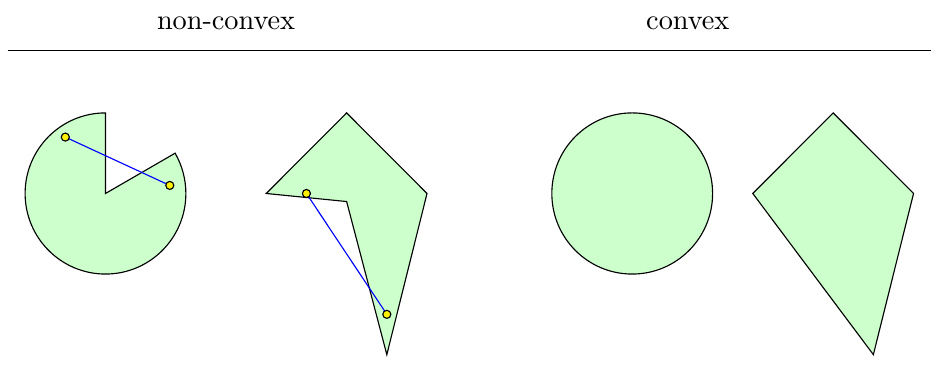
\includegraphics[scale=0.35]{cvx_noncvx}
\end{figure}

\begin{figure}
    \centering
    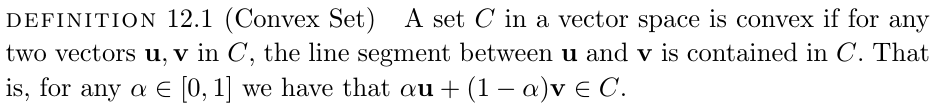
\includegraphics[scale=0.4]{cvx_set}
\end{figure}

\end{frame}

\begin{frame}
\frametitle{Convexity: Convex functions}

\begin{figure}
    \centering
    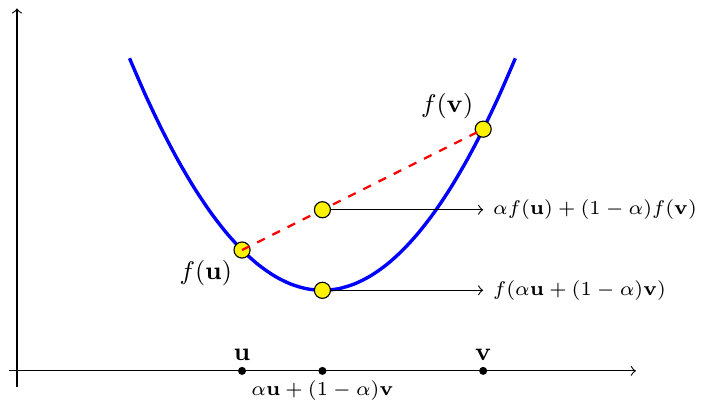
\includegraphics[scale=0.35]{cvx_fn}
\end{figure}

\begin{figure}
    \centering
    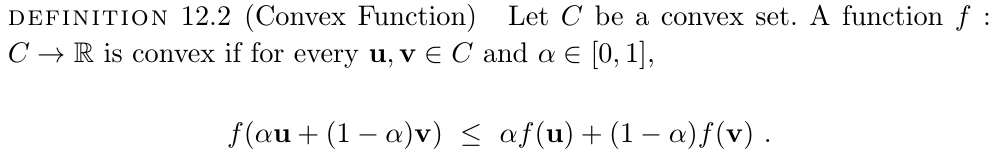
\includegraphics[scale=0.4]{cvx_fn_def}
\end{figure}

\end{frame}

\begin{frame}
\frametitle{Convexity: Convex functions}

Properties of convex fn:
\begin{itemize}
    \item  every local minimum is also a global minimum
    \item  for every $\mathbf{w}$ we can construct a tangent to $f$
    at $\mathbf{w}$ that lies below $f$ everywhere.
    If f is differentiable, this tangent is the linear function
    % $l(u) = f(w) + h∇f (w), u − wi$
\end{itemize}

\begin{figure}
    \centering
    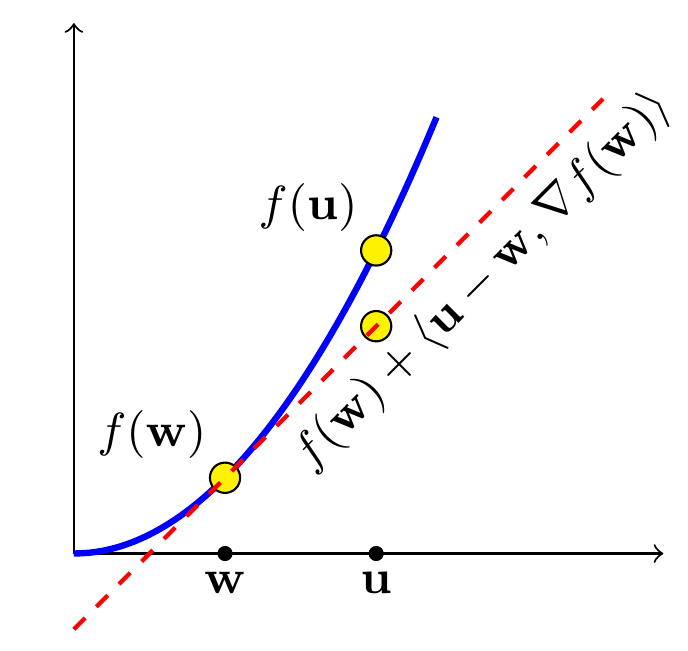
\includegraphics[scale=0.25]{cvx_fn_tangent}
\end{figure}

\end{frame}

\begin{frame}
\frametitle{Convexity: Convex functions}

\begin{figure}
    \centering
    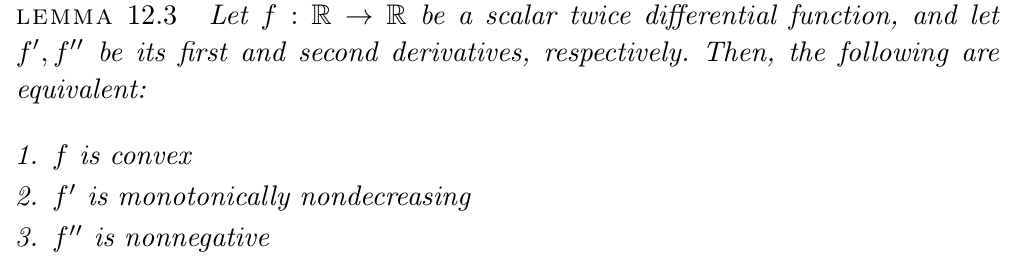
\includegraphics[scale=0.35]{lemma_12_3}
\end{figure}

\noindent\makebox[\linewidth]{\rule{\paperwidth}{0.4pt}}

\begin{figure}
    \centering
    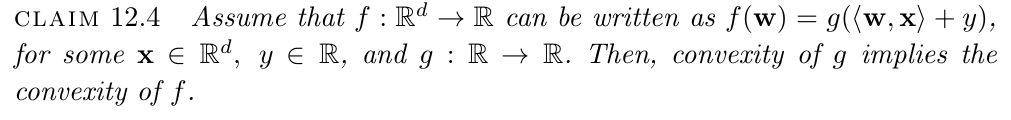
\includegraphics[scale=0.375]{claim_12_4}
\end{figure}

\noindent\makebox[\linewidth]{\rule{\paperwidth}{0.4pt}}

\begin{figure}
    \centering
    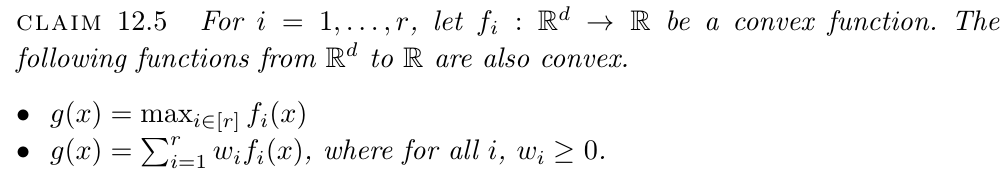
\includegraphics[scale=0.375]{claim_12_5}
\end{figure}

\end{frame}


\begin{frame}
\frametitle{Lipschitzness}
\begin{figure}
    \centering
    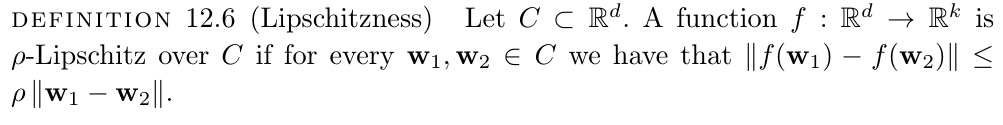
\includegraphics[scale=0.45]{def_12_6}
\end{figure}

Properties:
\begin{itemize}
    \item a Lipschitz function can \textbf{not} change too fast
    \item if the derivative of $f$ is everywhere bounded (in absolute value) by $\rho$,
        then the function is $\rho$-Lipschitz.
    \item \textbf{composition} of Lipschitz functions \textbf{preserves} Lipschitzness.
\end{itemize}

\end{frame}


\begin{frame}
\frametitle{Smoothness}
\begin{figure}
    \centering
    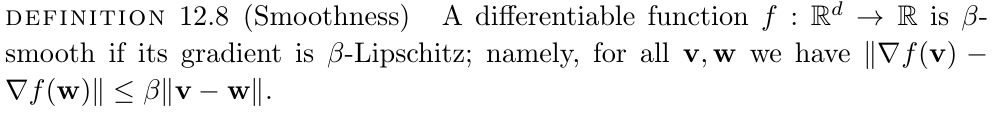
\includegraphics[scale=0.45]{def_12_8}
\end{figure}

Properties:
\begin{itemize}
    \item when a function is \textbf{both} convex and smooth,\\
        we have both \textbf{upper and lower bounds} on the difference between
        the function and its first order approximation.
    \item a \text{composition} of a smooth scalar function over a linear function \textbf{preserves} smoothness.
    \begin{figure}
        \centering
        
\includegraphics[scale=0.225]{claim_12_9}
    \end{figure}
\end{itemize}

\end{frame}

\section{Convex Learning Problems}
\frame{\tableofcontents[currentsection, hideothersubsections]}

% In general, a convex learning problem is a problem whose hypothesis class is a
% convex set, and whose loss function is a convex function for each example.

\begin{frame}
\frametitle{Convex Learning Problems: Intro}

Recall, we have:
\begin{itemize}
    \item a set of examples $\mathcal{Z} = \mathcal{X} \times \mathcal{Y}$
    \item a hypothesis class $\mathcal{H}$, which can be an arbitrary set,\\
    for now consider: $ \mathcal{H} \subseteq \mathbb{R}^d$,
    thus, denote a hypothesis in $\mathcal{H}$ by $\mathbf{w}$
    \item a loss function $\ell: \mathcal{H} \times \mathcal{Z} \mapsto \mathbb{R_{+}}$
\end{itemize}

\begin{figure}
    \centering
    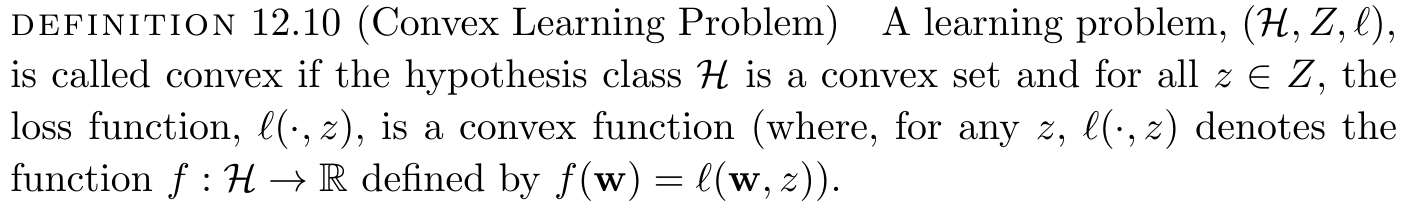
\includegraphics[scale=0.3]{def_12_10}
\end{figure}

\end{frame}

\begin{frame}
\frametitle{Convex Learning Problems: Intro}

Example 12.7: \\
Linear Regression with the Squared Loss
\begin{itemize}
    \item  to learn a linear function $h: \mathbb{R}^d \mapsto \mathbb{R}$ that best approximates
        the relationship between ``explanatory'' and outcome variables.
    \item Each linear function is parameterized by a vector $\mathbf{w} \in \mathbb{R}^d$,\\
        hence $\mathcal{H} = \mathbb{R}^d$
    \item set of examples:
    $\mathcal{Z} = \mathcal{X} \times \mathcal{Y} = \mathbb{R}^d \times \mathbb{R} = \mathbb{R}^{d+1}$
    \item loss function: $\ell(\mathbf{w}, (\mathbf{x}, y)) = (\langle \mathbf{w},\mathbf{x}  \rangle - y)^2$
    \item Clearly: $\mathcal{H}$ is a convex set and  $\ell$ is convex fn wrt $\mathbf{w}$
\end{itemize}

\begin{figure}
    \centering
    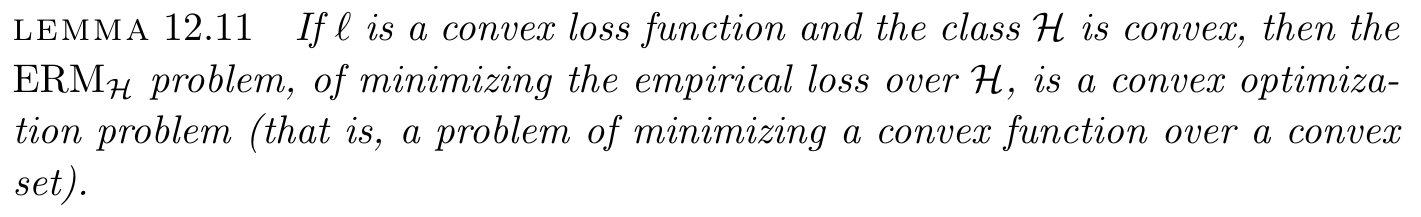
\includegraphics[scale=0.3]{lemma_12_11}
\end{figure}

\end{frame}

\begin{frame}
\frametitle{Convex Learning Problems: Learnability}
QUESTIONS:
\begin{itemize}
    \item is convexity a sufficient condition for the learnability of a problem?
    \item are all convex learning problems over $R^d$ learnable?
\end{itemize}
\vspace{5mm}

ANSWERS:\\
\begin{itemize}
    \item \textbf{not all} convex learning problems over $\mathbb{R}^d$ are learnable.
    \item Convex problems are \textbf{learnable under} some restricting conditions:\\
        the properties of convexity, boundedness, and Lipschitzness or smoothness
        of the loss function are sufficient for learnability.
\end{itemize}

\end{frame}

\begin{frame}
\frametitle{Convex Learning Problems: Learnability}
TWO families of learning problems are learnable.

\noindent\makebox[\linewidth]{\rule{\paperwidth}{0.4pt}}

\begin{figure}
    \centering
    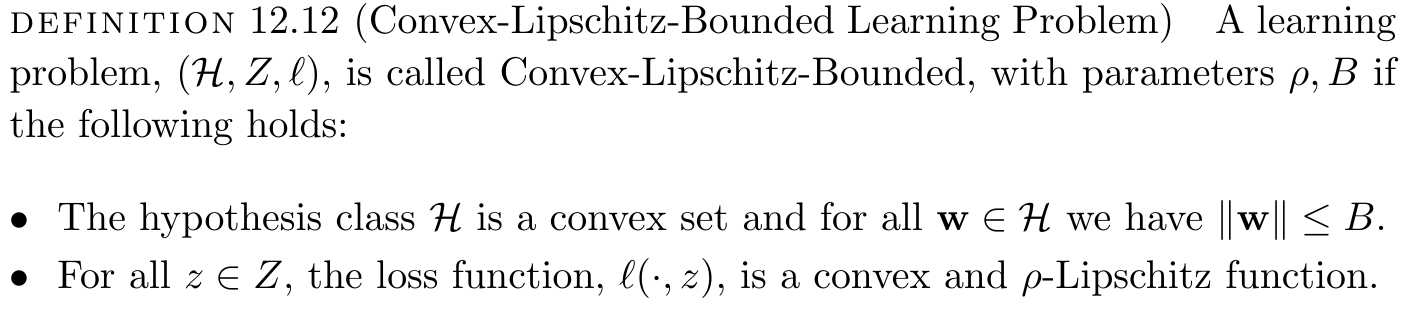
\includegraphics[scale=0.3]{def_12_12}
\end{figure}

\noindent\makebox[\linewidth]{\rule{\paperwidth}{0.4pt}}

\begin{figure}
    \centering
    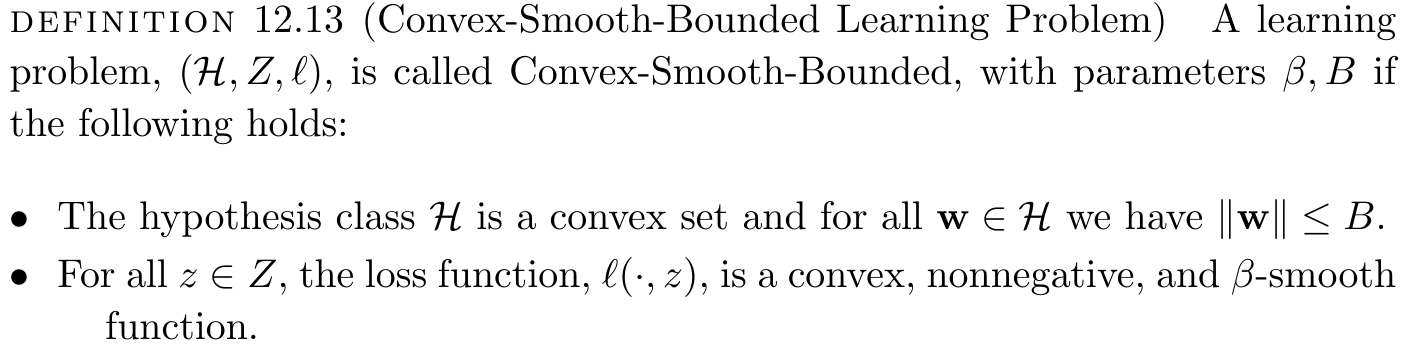
\includegraphics[scale=0.3]{def_12_13}
\end{figure}

\end{frame}



\section{Surrogate Loss Function}
\frame{\tableofcontents[currentsection, hideothersubsections]}

\begin{frame}
\frametitle{Surrogate Loss Fn: Intro}

WHAT:\\
handle some \textbf{non}convex problems
by minimizing ``surrogate'' loss functions that are \text{convex}
\vspace{4mm}

WHY:\\
the natural loss function is not convex, e.g.  $0-1$ loss
\vspace{4mm}

HOW:\\
to upper bound the nonconvex loss function by a convex surrogate loss function
that
\begin{itemize}
    \item are convex
    \item upper bounds the original loss.
\end{itemize}
\end{frame}

\begin{frame}
\frametitle{Surrogate Loss Fn: Example}
In the context of learning halfspaces:\\
Hinge loss as a convex surrogate for the $0-1$ loss
\footnote{{\tiny https://scicomp.stackexchange.com/questions/5628/confusion-related-to-convexity-of-0-1-loss-function}}

\begin{figure}
    \centering
    
\includegraphics[scale=0.25]{eq_hinge_loss}
\end{figure}

\begin{figure}
    \centering
    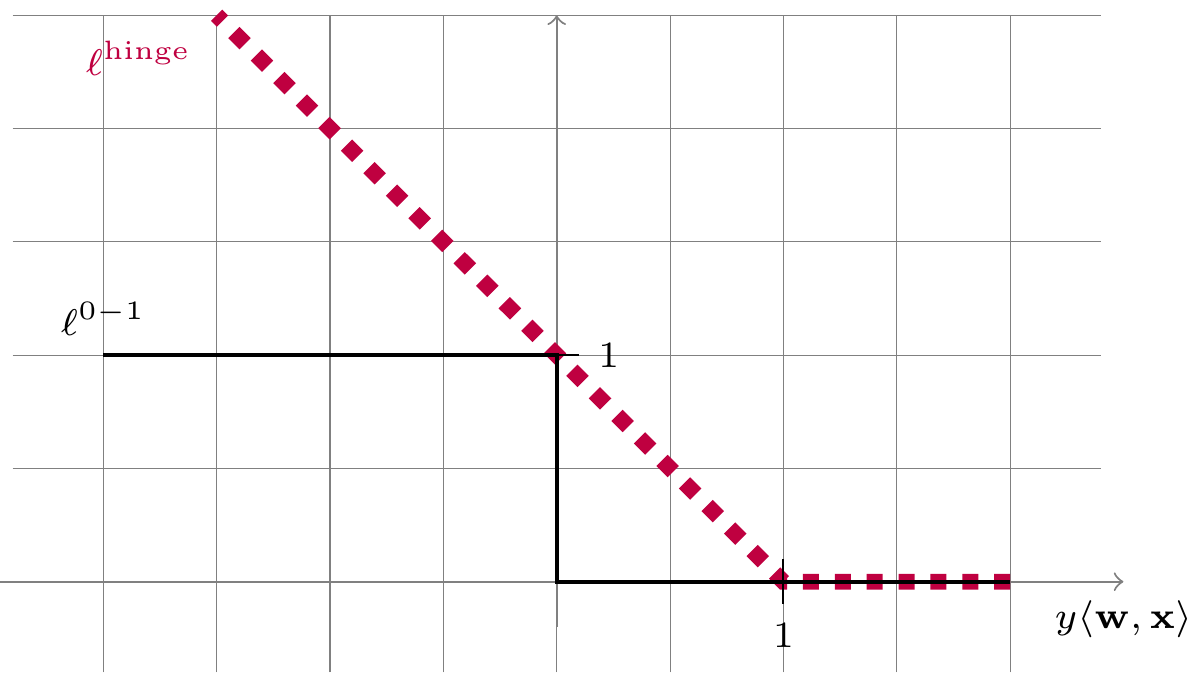
\includegraphics[scale=0.25]{fig_surr_fn}
\end{figure}

\end{frame}




\section{Gradient Descent}
\frame{\tableofcontents[currentsection, hideothersubsections]}

\begin{frame}
\frametitle{Gradient Descent: Intro}

Recall:\\
\begin{itemize}
    \item hypotheses as vectors $\mathbf{w}$ that \\
         come from a convex hypothesis class, $\mathcal{H}$
    \item goal of learning:\\
          to minimize the risk function $L_D(\mathbf{w})$;\\
          \textbf{not} the empirical risk $L_S (h)$
    \item gradient def:
        \begin{figure}
            \centering
            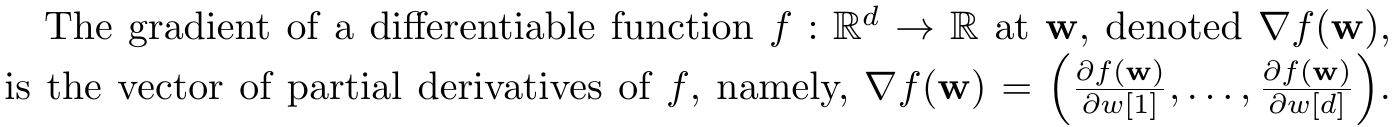
\includegraphics[scale=0.30]{grad_def_p185}
        \end{figure}
\end{itemize}

\end{frame}

\begin{frame}
\frametitle{Gradient Descent: Intro}
Gradient descent:
\begin{itemize}
\item an iterative optimization procedure
\item at each step: \\
    improve the solution by
    taking a step along the negative of the gradient of the function to be minimized at the current point

    \begin{figure}
    \centering
    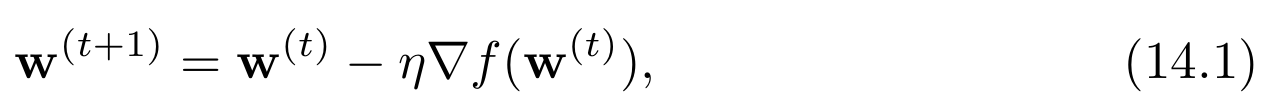
\includegraphics[scale=0.30]{eq_14_1}
    \end{figure}
\item after $T$ iterations, output either
    \begin{itemize}
        \item averaged vector
            \footnote{taking the average turns out to be rather useful, especially
            when we generalize gradient descent to nondifferentiable functions and to the stochastic case}, \textbf{or}
        \item last vector, \textbf{or}
        \item the best performing vector
    \end{itemize}
\end{itemize}

\end{frame}

\begin{frame}
\frametitle{Gradient Descent: Analysis of GD for Convex-Lipschitz Fn}

LET:
\begin{itemize}
\item $\mathbf{w^*}$ be any vector and
\item $B$ be an upper bound on $\parallel \mathbf{w^*} \parallel$
\end{itemize}
\vspace{5mm}

GOAL:\\
to obtain an upper bound on  $f(\bar{\mathbf{w}}) - f(\mathbf{w^*})$,
where $\bar{\mathbf{w}} = \frac{1}{T} \sum_{1}^{T} \mathbf{w}^{(t)}$
\vspace{5mm}

RESULT:\\
From the definition of $\bar{\mathbf{w}}$, and using Jensen's inequality, we obtain:
\begin{figure}
    \centering
    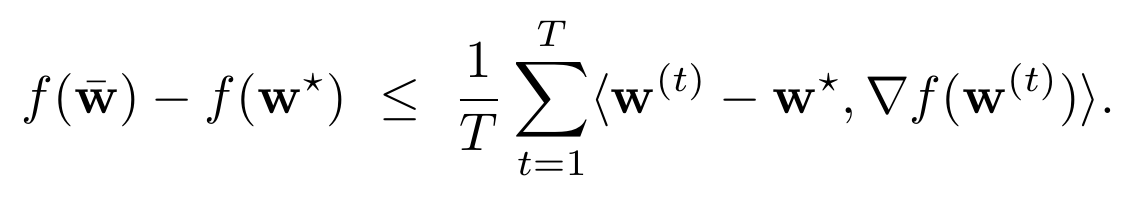
\includegraphics[scale=0.25]{eq_14_3b}
\end{figure}

\end{frame}

\begin{frame}
\frametitle{Gradient Descent: Analysis of GD for Convex-Lipschitz Fn}

\begin{figure}
    \centering
    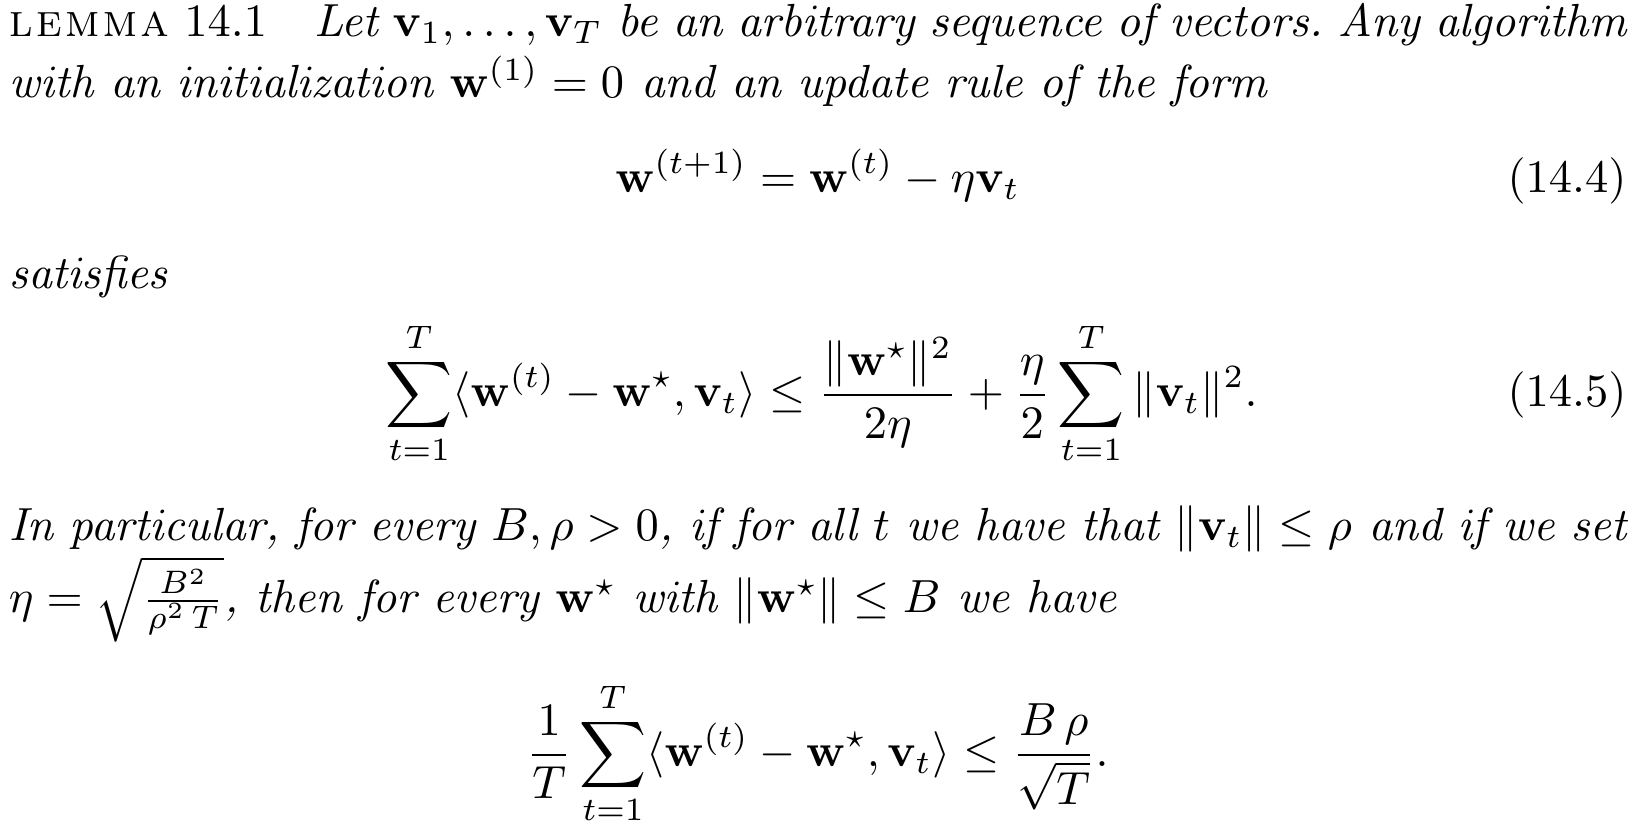
\includegraphics[scale=0.25]{lemma_14_1}
\end{figure}

\end{frame}

\begin{frame}
\frametitle{Gradient Descent: Analysis of GD for Convex-Lipschitz Fn}

\begin{figure}
    \centering
    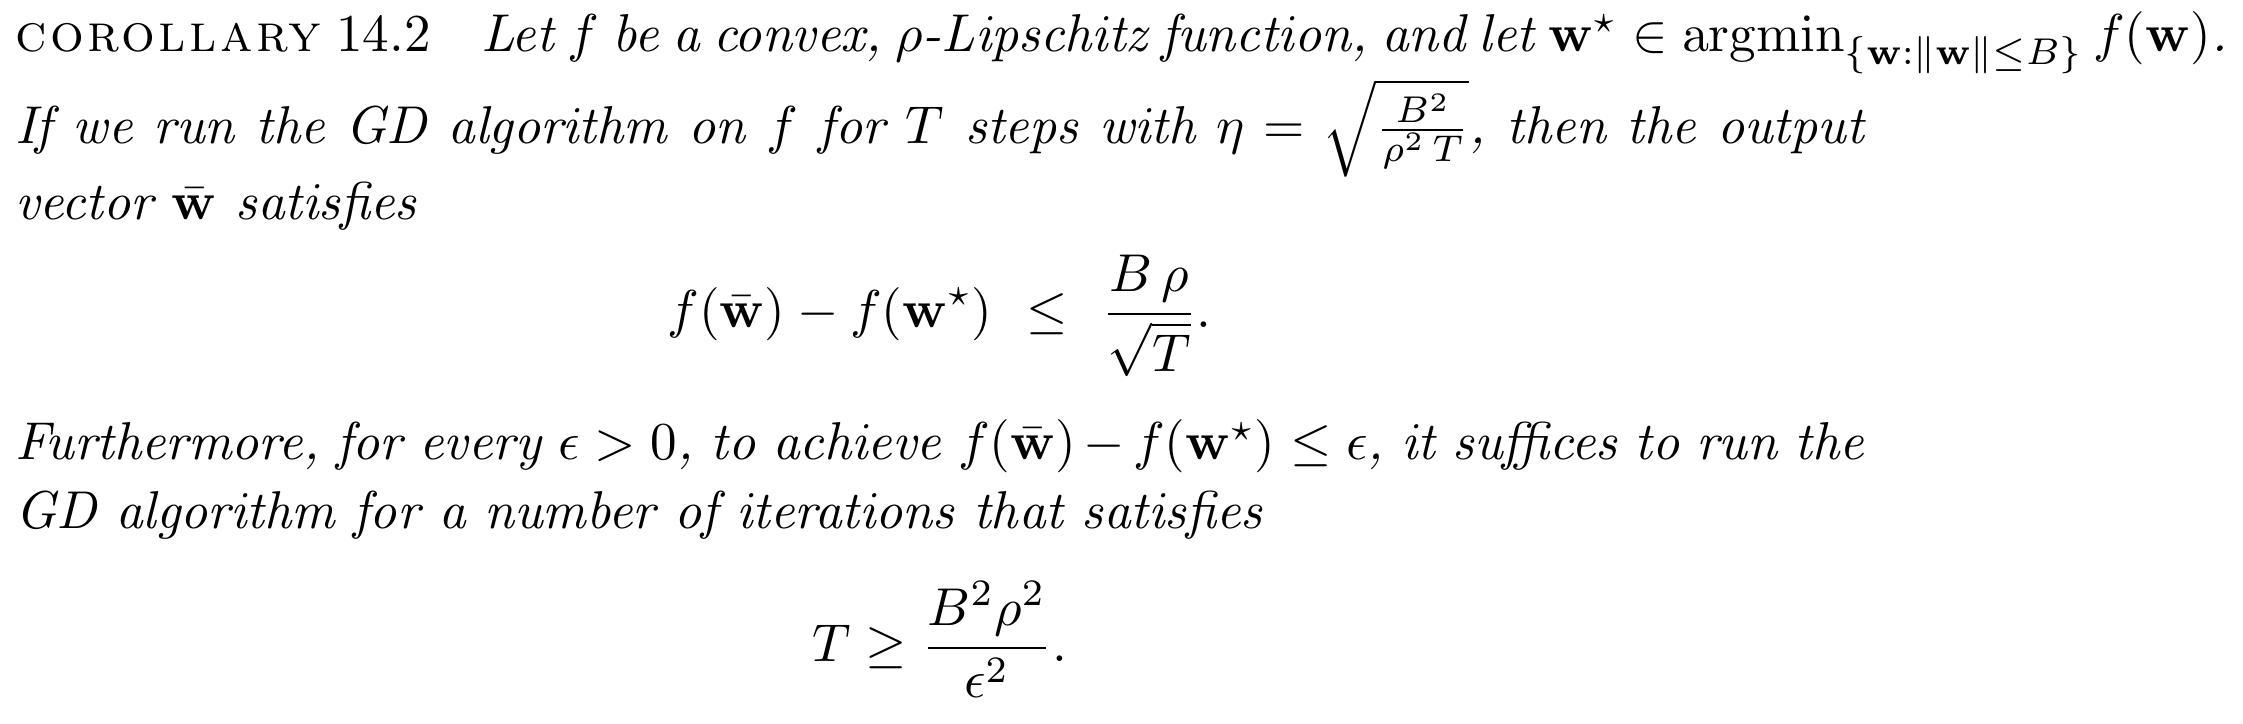
\includegraphics[scale=0.2]{corollary_14_2}
\end{figure}

\end{frame}

\section{Subgradients}
\frame{\tableofcontents[currentsection, hideothersubsections]}

\begin{frame}
\frametitle{Subgradients: Intro}

WHAT:\\
apply GD to \textbf{non}differentiable convex function
\vspace{5mm}

HOW:\\
use subgradient of $f(\mathbf{w})$ at $\mathbf{w}^{(t)}$, instead of the gradient;\\
(the analysis of the convergence rate remains unchanged)

\end{frame}

\begin{frame}
\frametitle{Subgradients: Intro}

\begin{figure}
    \centering
    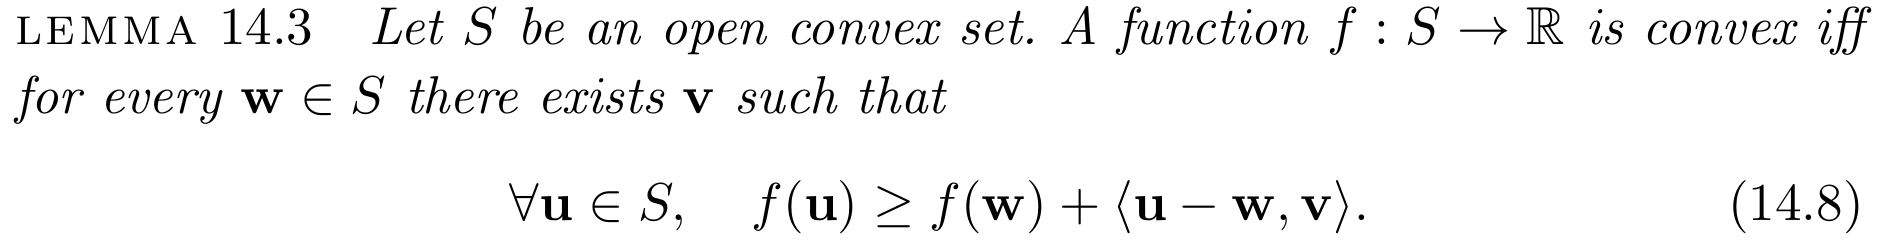
\includegraphics[scale=0.225]{lemma_14_3}
\end{figure}

\noindent\makebox[\linewidth]{\rule{\paperwidth}{0.4pt}}

\begin{figure}
    \centering
    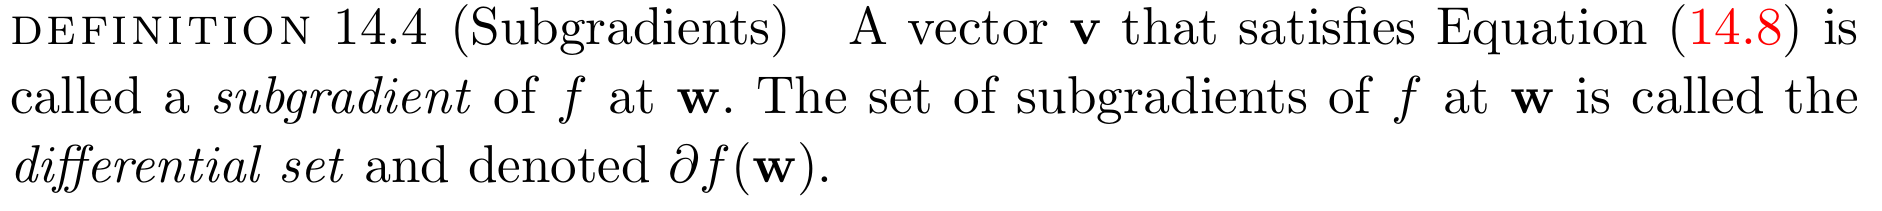
\includegraphics[scale=0.225]{def_14_4}
\end{figure}

\end{frame}

\begin{frame}
\frametitle{Subgradients: Intro}

\begin{figure}
    \centering
    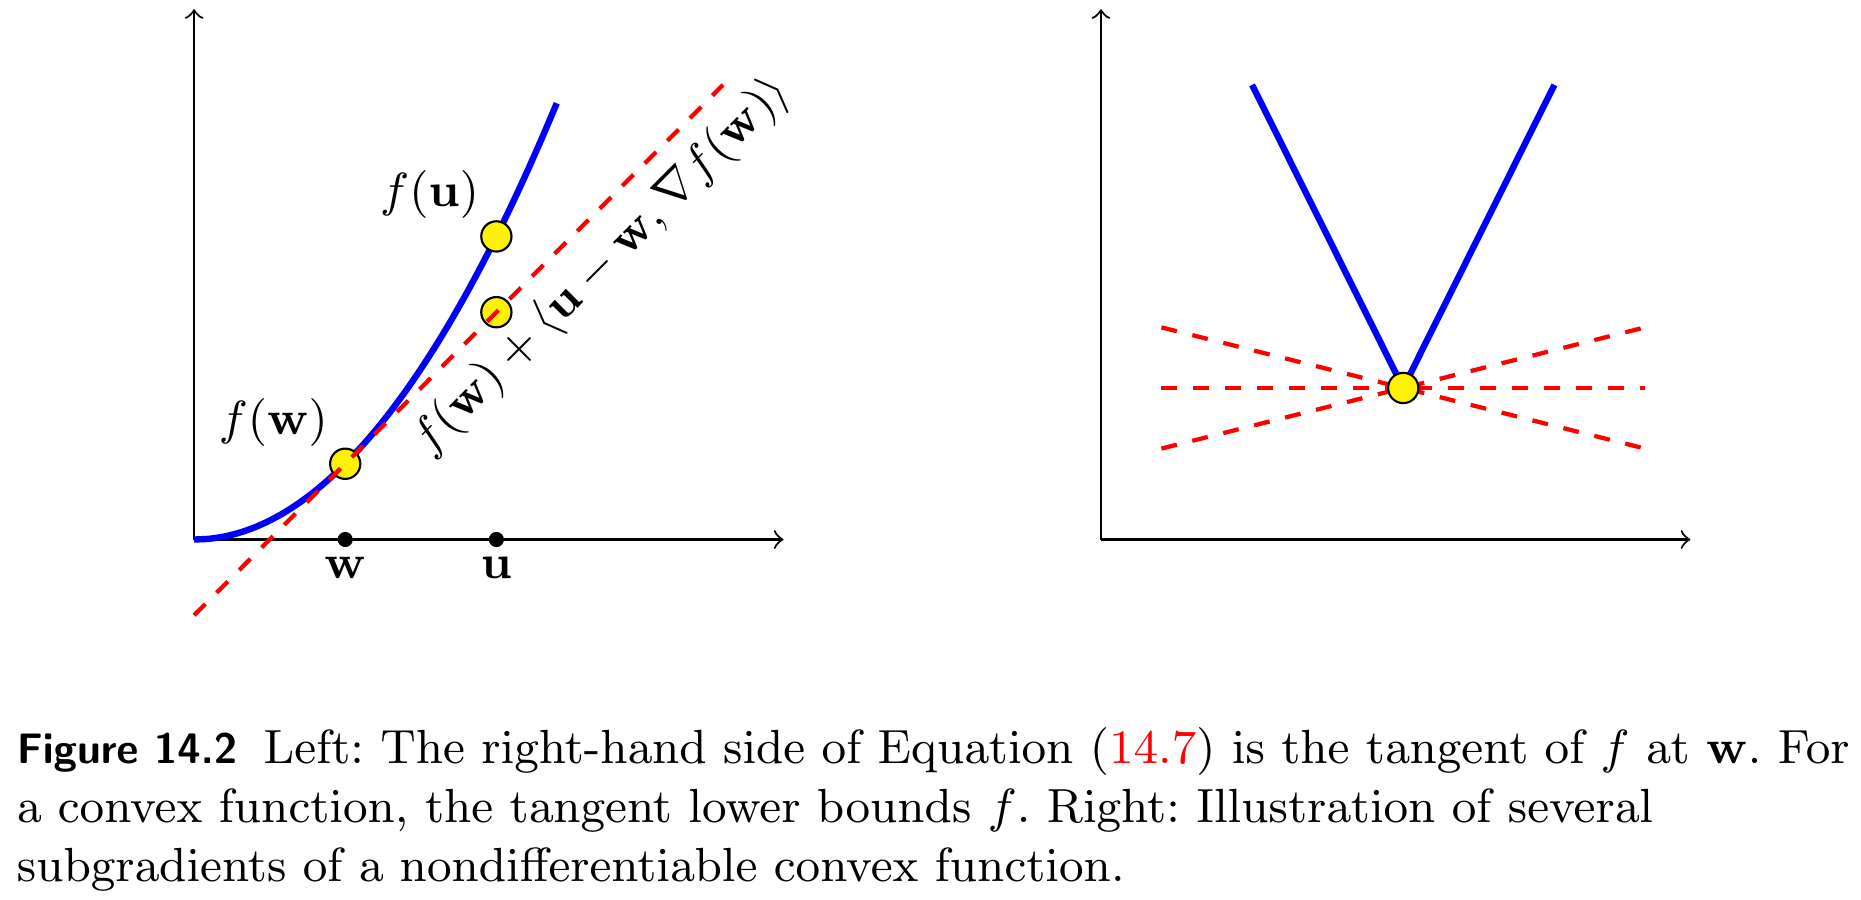
\includegraphics[scale=0.25]{fig_14_2}
\end{figure}

\end{frame}

\begin{frame}
\frametitle{Subgradients: Calculating Subgradients}

How do we construct subgradients of a given convex function?
\vspace{5mm}

For pointwise maximum functions:
\begin{figure}
    \centering
    
\includegraphics[scale=0.225]{claim_14_6}
\end{figure}

\begin{figure}
    \centering
    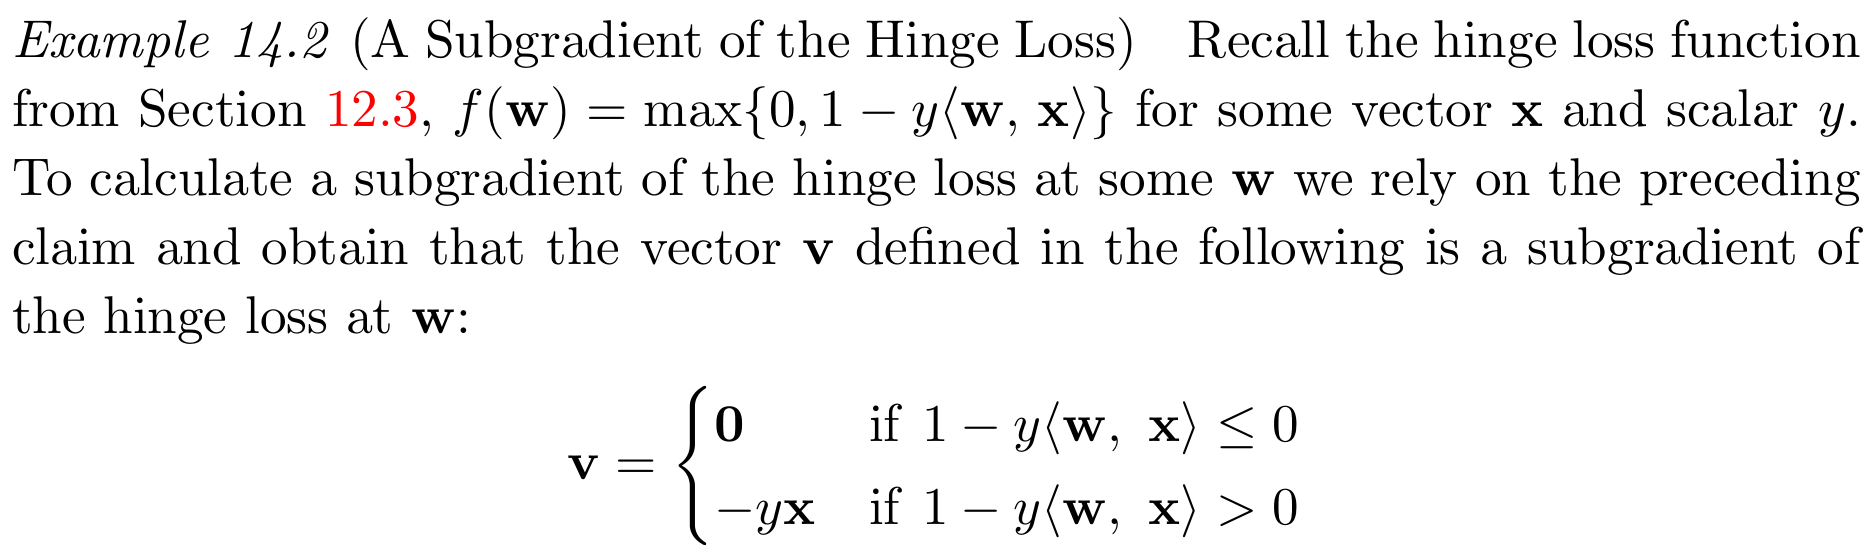
\includegraphics[scale=0.225]{example_14_2}
\end{figure}

\end{frame}

\section{Stochastic Gradient Descent (SGD)}
\frame{\tableofcontents[currentsection, hideothersubsections]}

\begin{frame}
\frametitle{SGD: Intro}

WHAT:\\
Stochastic Gradient Descent (SGD);
\vspace{5mm}

WHY:\\
do not know $D$, so do not know the gradient of $L_D(w)$.
\vspace{5mm}

HOW:\\
take a step along a \textbf{random} direction (vector), as long as \\
its \textbf{expected value} at each iteration will \textbf{equal the gradient direction} \\
(more generally, a subgradient of the function at the current vector)
\end{frame}

\begin{frame}
\frametitle{SGD: Intro}

\begin{figure}
    \centering
    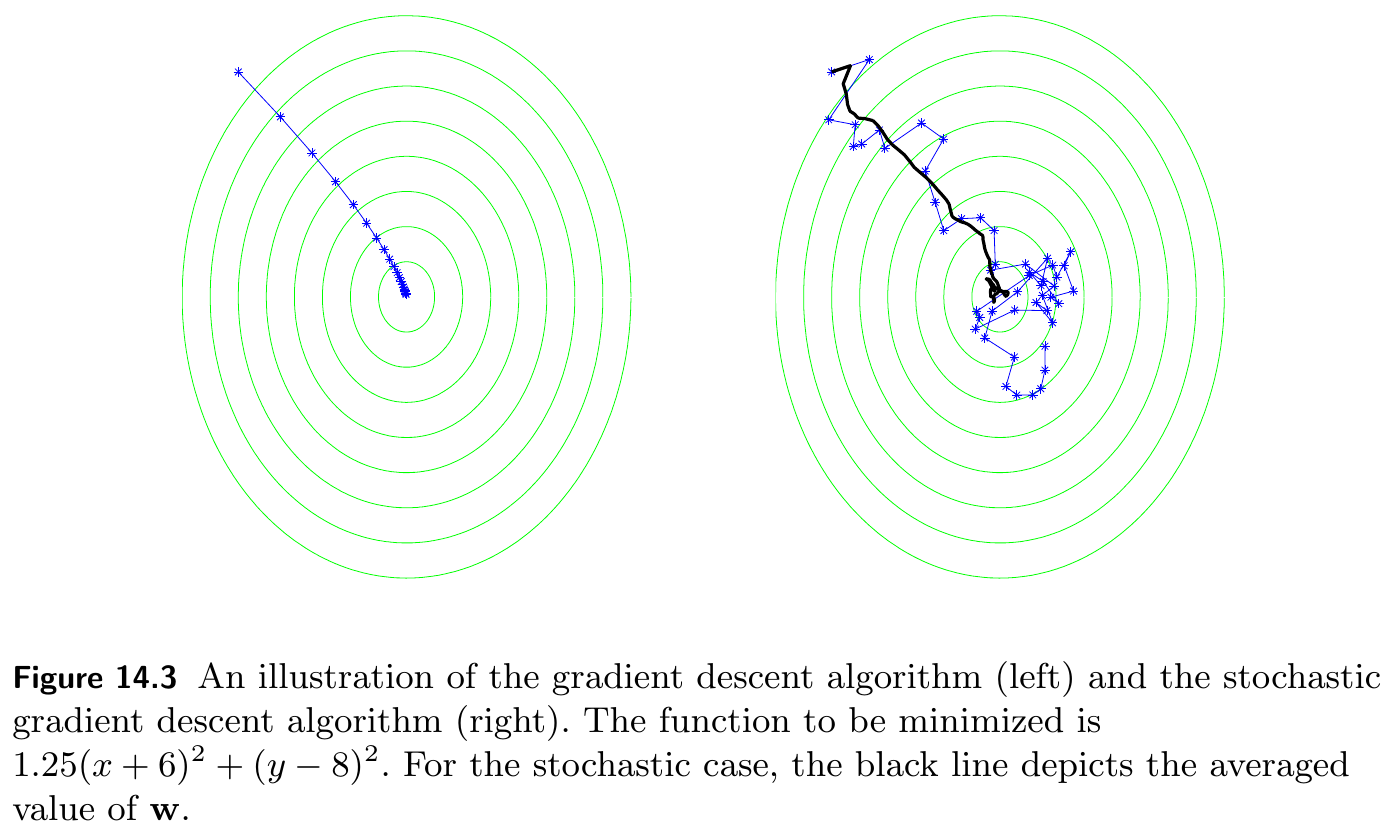
\includegraphics[scale=0.3]{fig_14_3}
\end{figure}

\end{frame}

\begin{frame}
\frametitle{SGD: Intro}

\begin{figure}
    \centering
    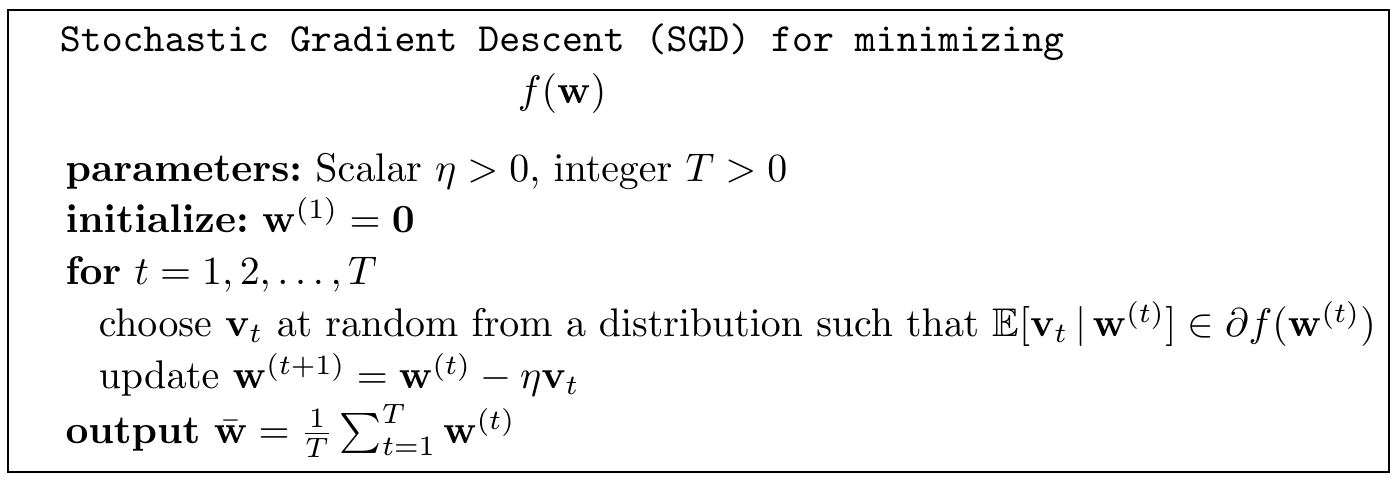
\includegraphics[scale=0.325]{sgd}
\end{figure}

\end{frame}



\begin{frame}
\frametitle{SGD: Analysis for Convex-Lipschitz-Bounded Fn}

\begin{figure}
    \centering
    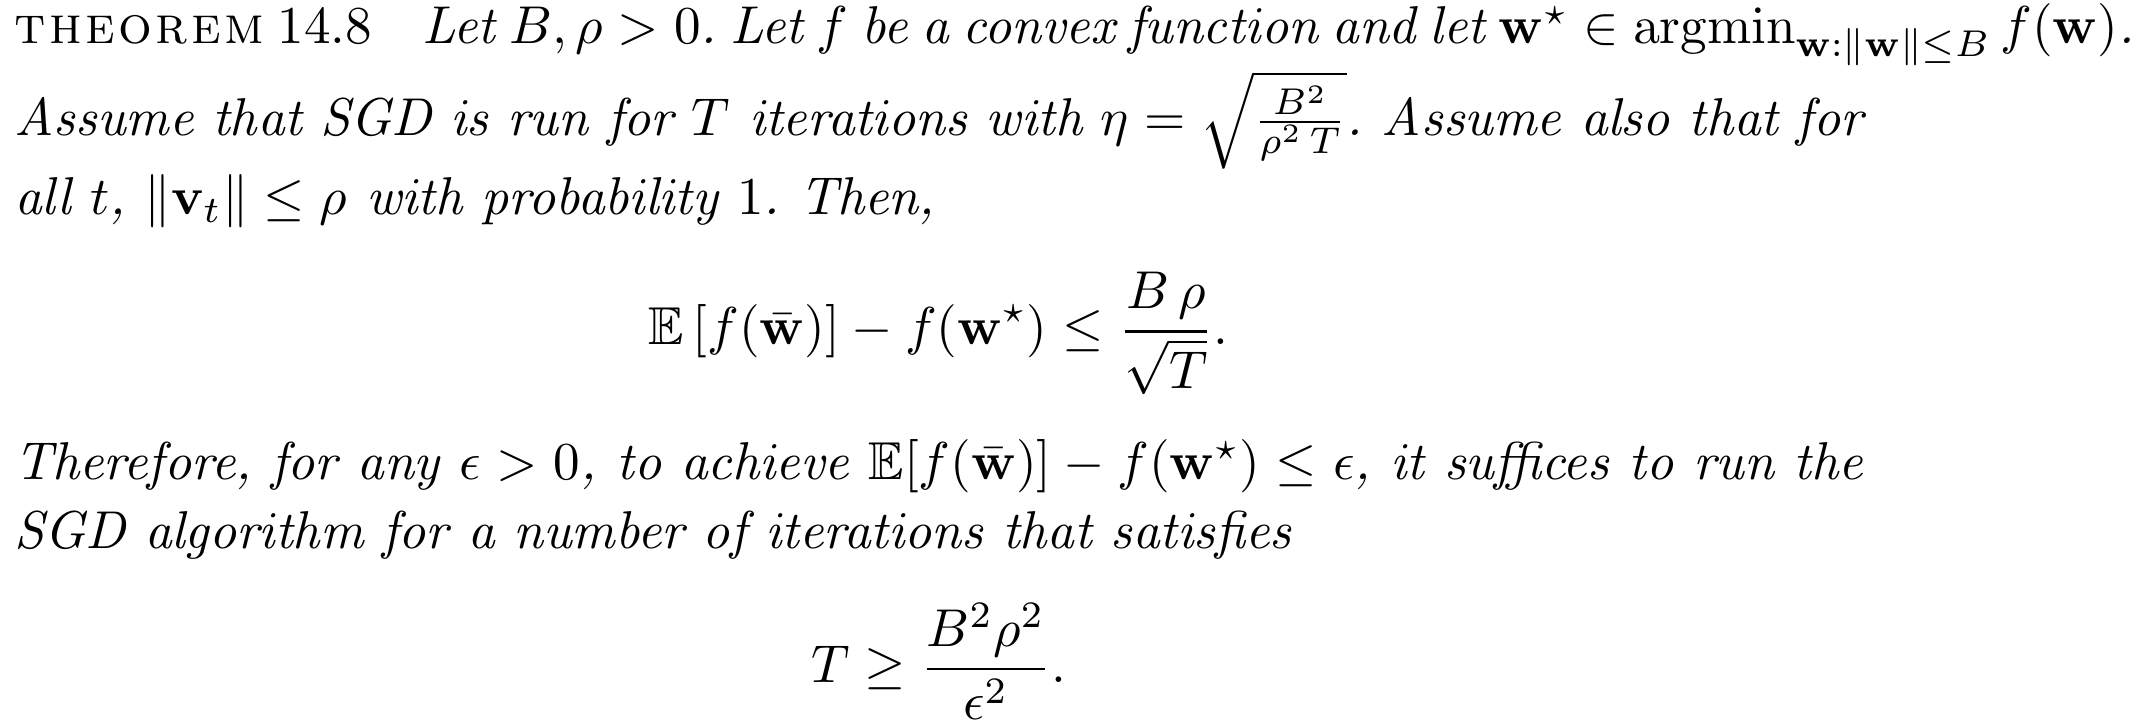
\includegraphics[scale=0.2]{theorem_14_8}
\end{figure}

\end{frame}

\section{Learning with SGD}
\frame{\tableofcontents[currentsection, hideothersubsections]}

\begin{frame}
\frametitle{Learning with SGD: Risk Minimization}

Recall, in learning:\\
\begin{itemize}
\item want to minimize the risk function, $L_D(\mathbf{w}) = \mathbb{E}_{z \sim D} [\ell(\mathbf{w}, z)]$
\item do not know $D$, so cannot simply calculate $\nabla L_D (\mathbf{w}^{(t)} )$
\item as an estimate to minimizing $L_D(w)$: minimize $L_S(w)$~\footnote{empirical risk}
\end{itemize}
\vspace{5mm}

SGD minimizes $L_D(w)$ directly:\\
find an \textbf{unbiased estimate} of the gradient of $L_D(\mathbf{w})$, that is,\\
a random vector whose conditional expected value is $\nabla L_D (\mathbf{w}^{(t)} )$

\end{frame}


\begin{frame}
\frametitle{Learning with SGD: Risk Minimization}

Construction of the random vector $\mathbf{v}_t$ for  a differentiable risk fn $L_D$:
\begin{itemize}
\item sample $z \sim D$
\item define $\mathbf{v}_t$ to be the gradient of $\ell(\mathbf{w}, z)$ wrt $\mathbf{w}$, at $\mathbf{w}^{(t)}$
\item by the linearity of the gradient we have:
    \begin{figure}
        \centering
        
\includegraphics[scale=0.25]{eq_14_13}
    \end{figure}
\end{itemize}
\vspace{5mm}

Thus, the gradient of the loss function $\ell(w, z)$ at $\mathbf{w}^{(t)}$ is
\begin{itemize}
\item unbiased estimate of the gradient of the risk function $L_D( w^{(t)} )$ and
\item constructed by sampling a single fresh example $z \sim D$ at each iteration $t$.
\end{itemize}

\end{frame}


\begin{frame}
\frametitle{Learning with SGD: Risk Minimization}

\begin{figure}
    \centering
    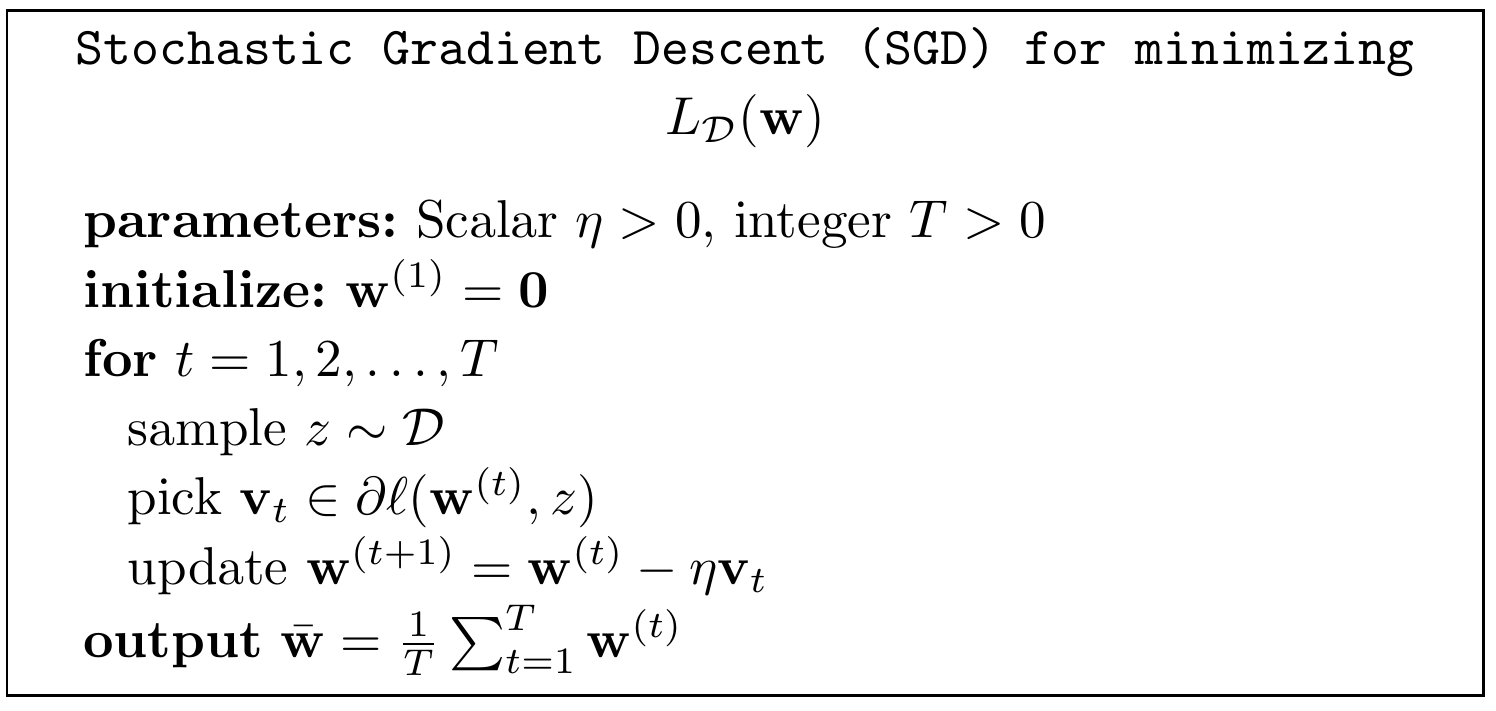
\includegraphics[scale=0.25]{sgd2}
\end{figure}

Same for nondifferentiable loss functions,\\
simply let $\mathbf{v}_t$ be a subgradient of $\ell(\mathbf{w}, z)$ at $\mathbf{w}^{(t)}$

\end{frame}

\begin{frame}
\frametitle{Learning with SGD: Convex-Smooth Learning Problems}

\begin{figure}
    \centering
    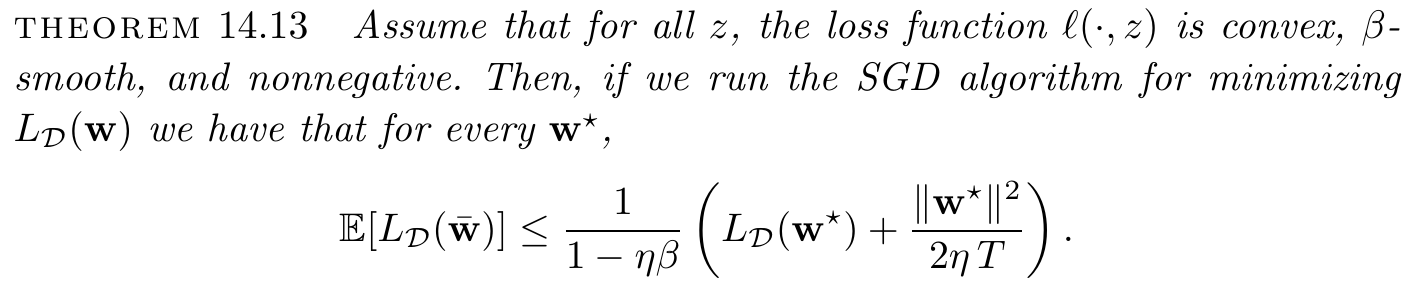
\includegraphics[scale=0.25]{theorem_14_13}
\end{figure}

\begin{figure}
    \centering
    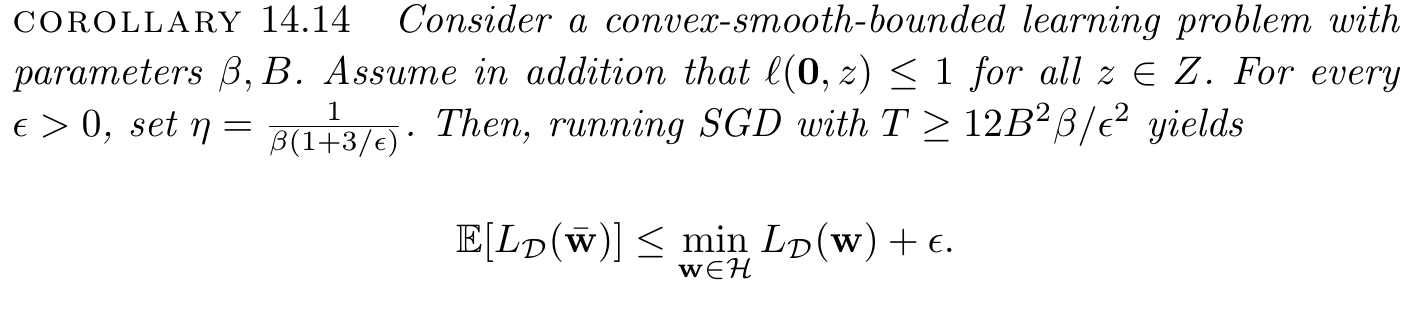
\includegraphics[scale=0.25]{corollary_14_14}
\end{figure}

\end{frame}

\begin{frame}
\frametitle{Learning with SGD: Regularized Loss Minimization}

WHAT:\\
to solve the regularized loss minimization:
\begin{figure}
    \centering
    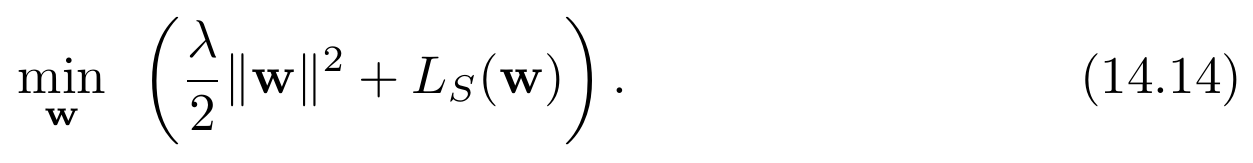
\includegraphics[scale=0.25]{eq_14_14}
\end{figure}

WHY:\\
\begin{itemize}
\item SGD enjoys the same worst-case sample complexity bound as regularized loss minimization
\item on some distributions, regularized loss minimization may yield a better solution.
\end{itemize}

HOW:\\
...
\end{frame}

\begin{frame}
\frametitle{Learning with SGD: Regularized Loss Minimization}

WHAT:\\
to solve the regularized loss minimization:
\begin{figure}
    \centering
    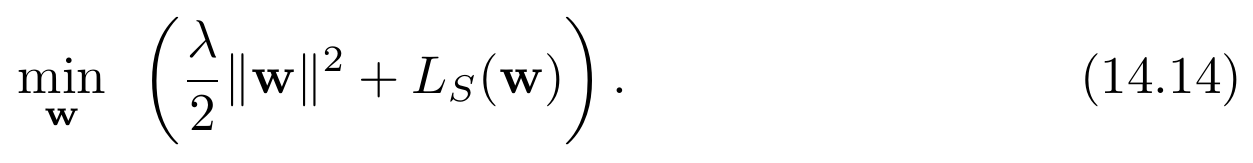
\includegraphics[scale=0.25]{eq_14_14}
\end{figure}

HOW:\\
\begin{itemize}
\item define $f(\mathbf{w}) = \frac{\lambda}{2} \parallel w \parallel^2 + L_S(\mathbf{w})$.
    \begin{itemize}
        \item $f$ is a $\lambda$-strongly convex function;
        \item therefore, apply the SGD variant with $\mathcal{H} = \mathbb{R}^d$.
    \end{itemize}
\item construct an unbiased estimate of a subgradient of $f$ at $\mathbf{w}^{(t)}$
    \begin{itemize}
        \item pick $z$ uniformly at random from $S$,
        \item choose $\mathbf{v}_t$ in $\partial \ell(\mathbf{w}^{(t)}, z)$
        \item (then) the expected value of $\lambda \mathbf{w}^{(t)} + \mathbf{v}t$ is a subgradient of f at $\mathbf{w}^{(t)}$.
    \end{itemize}
\end{itemize}

\end{frame}


\section{Conclusions}
\frame{\tableofcontents[currentsection, hideothersubsections]}

\begin{frame}
\frametitle{Conclusions}
?
\end{frame}

\begin{frame}
\Huge{\centerline{Discussion time and thank you.}}
\end{frame}
\begin{frame} [allowframebreaks]
\frametitle{References}
{\tiny
\bibliographystyle{apacite}
\bibliography{ref}
}
\end{frame}

\begin{frame}
\Huge{\centerline{Discussion time and thank you.}}
\end{frame}

%%%%%%%%%%%%%%%%%%%%%%%%%%%%%%%%%%%%%%%%%%%%%%%%%%%%%%%%%%%%%%%%%%%%%%%%%%%%%%%

\end{document}
